\documentclass[twoside,11pt]{article}
\usepackage[ngerman,english]{babel}
\usepackage{csquotes}

\usepackage{geometry}
\geometry{a4paper, top=30mm, bottom=35mm, inner=25mm, outer=25mm, footskip=18.8mm}

\usepackage{caption}
\usepackage{subcaption}

% Zeilenabstand etwas vergroessert (1.1)
\usepackage[onehalfspacing]{setspace}
\setstretch{1.1}

\usepackage[hidelinks]{hyperref}



\usepackage{mathtools, amssymb, amsthm}
\allowdisplaybreaks
\usepackage{tensor}
\usepackage{braket}
\usepackage{enumitem}

% biblatex https://www.overleaf.com/learn/latex/Bibliography_management_with_biblatex
% https://tex.stackexchange.com/questions/12806/guidelines-for-customizing-biblatex-styles
\usepackage[
  backend=biber,
  sorting=nty,
  maxbibnames=50,
  maxcitenames=4,
  style=alphabetic,
  giveninits=true,
  isbn=false,
]{biblatex}
\addbibresource{refs.bib}

\hypersetup{
    colorlinks=true,
    linkcolor=violet,
    urlcolor=blue,
    citecolor=[rgb]{0,0.6,0},
    }

\iffalse
\hypersetup{%
    ,urlcolor=black
    ,citecolor=black
    ,linkcolor=black
    }
\fi

% new page at every new section (https://tex.stackexchange.com/questions/9497/start-new-page-with-each-section, there's another probably better answer here)
\AddToHook{cmd/section/before}{\clearpage}


\usepackage{graphicx}


\usepackage{xcolor}
%\newcommand{\red}[1]{\textcolor{red}{#1}}
\newcommand{\red}[1]{#1}

\theoremstyle{plain}

\newtheorem{theorem}{\textsc{Theorem}}[section]
\newtheorem{lemma}[theorem]{\textsc{Lemma}}
\newtheorem{proposition}[theorem]{\textsc{Proposition}}
\newtheorem{corollary}[theorem]{\textsc{Corollary}}
\newtheorem{conjecture}[theorem]{\textsc{Conjecture}}
\newtheorem{definition}[theorem]{\textsc{Definition}}

\theoremstyle{definition}
\newtheorem{remark}[theorem]{\textsc{Remark}}
\newtheorem{example}[theorem]{\textsc{Example}}

% https://tex.stackexchange.com/questions/248757/ntheorem-numbering-of-claim-and-its-proof

\newtheorem{claim}{Claim}[theorem]
\newtheorem*{unnumberedclaim}{Claim}

%\newtheorem{step}{Step}[theorem]

\newcommand{\step}[1]{\textbf{#1}\hspace{.5em}}

\theoremstyle{definition}
\usepackage{xifthen} % provides \isempty test

\renewcommand{\setminus}{\smallsetminus}

\let\Im\relax
\DeclareMathOperator{\Im}{Im}
\let\Re\relax
\DeclareMathOperator{\Re}{Re}

\newcommand{\1}{\mathbb{1}}
\newcommand{\actson}{\curvearrowright}
\newcommand{\inclusion}{\hookrightarrow}

\newcommand{\Cov}{\mathrm{Cov}}
\newcommand{\Var}{\mathrm{Var}}

% spaces, number groups etc.
\newcommand{\K}{\mathbb{K}}
\newcommand{\N}{\mathbb{N}}
\newcommand{\Z}{\mathbb{Z}}
\newcommand{\Q}{\mathbb{Q}}
\newcommand{\R}{\mathbb{R}}
\newcommand{\C}{\mathbb{C}}

%\renewcommand{\bar}{\widebar}

\DeclareMathOperator{\res}{res}

\newcommand{\diag}{\mathrm{diag}}
\newcommand{\End}{\mathrm{End}}
\newcommand{\Hom}{\mathrm{Hom}}
\newcommand{\Aut}{\mathrm{Aut}}
\newcommand{\Ext}{\mathrm{Ext}}
\newcommand{\Tor}{\mathrm{Tor}}

\DeclareMathOperator{\id}{id}
\DeclareMathOperator{\Id}{Id}
\DeclareMathOperator{\tr}{tr}
\DeclareMathOperator{\Tr}{\tr}
\DeclareMathOperator{\sgn}{sgn}
\DeclareMathOperator{\rk}{rk}
\DeclareMathOperator{\grad}{grad}

\DeclareMathOperator{\im}{im}
\DeclareMathOperator{\coker}{coker}

% probability
\newcommand{\E}{\mathbb{E}}

%\usepackage[default]{fontsetup} % to set the font to New Computer Modern, pdfLaTeX not allowed

\title{Machine Learning}

\begin{document}
\maketitle
\tableofcontents

\section{Machine Learning Basics}
\subsection{Bias-Variance tradeoff}
$$ Y = f(X) + \epsilon $$
where $\epsilon$ is random noise term with expectation 0 and variance $\sigma^2$.
The bias-variance decomposition breaks down the expected squared error $\E[(Y-\hat f(X))^2]$ into distinct components.

Crucially, the function $\hat f$ (I do not mean $\hat f(X)$!) is random, depending on the random training data $D = \{(x_1,y_1), \dots, (x_n,y_n)\}$.

Ultimately,
$$ \E[(Y-\hat f(X))^2 \mid X] = (f(X)-\E[\hat f(X) \mid X])^2 + \Var(\hat f(X) \mid X) + \sigma^2 $$
bias squared + variance + irreducible error

More readable,
$$ \E[(f(x)+\epsilon - \hat f(x))^2] = (f(x) - \E[\hat f(x)])^2 + \Var(\hat f(x)) + \sigma^2 $$
where, in the expectations, all randomness comes from $D$ and $\epsilon$, not from $X$.

\begin{center}
    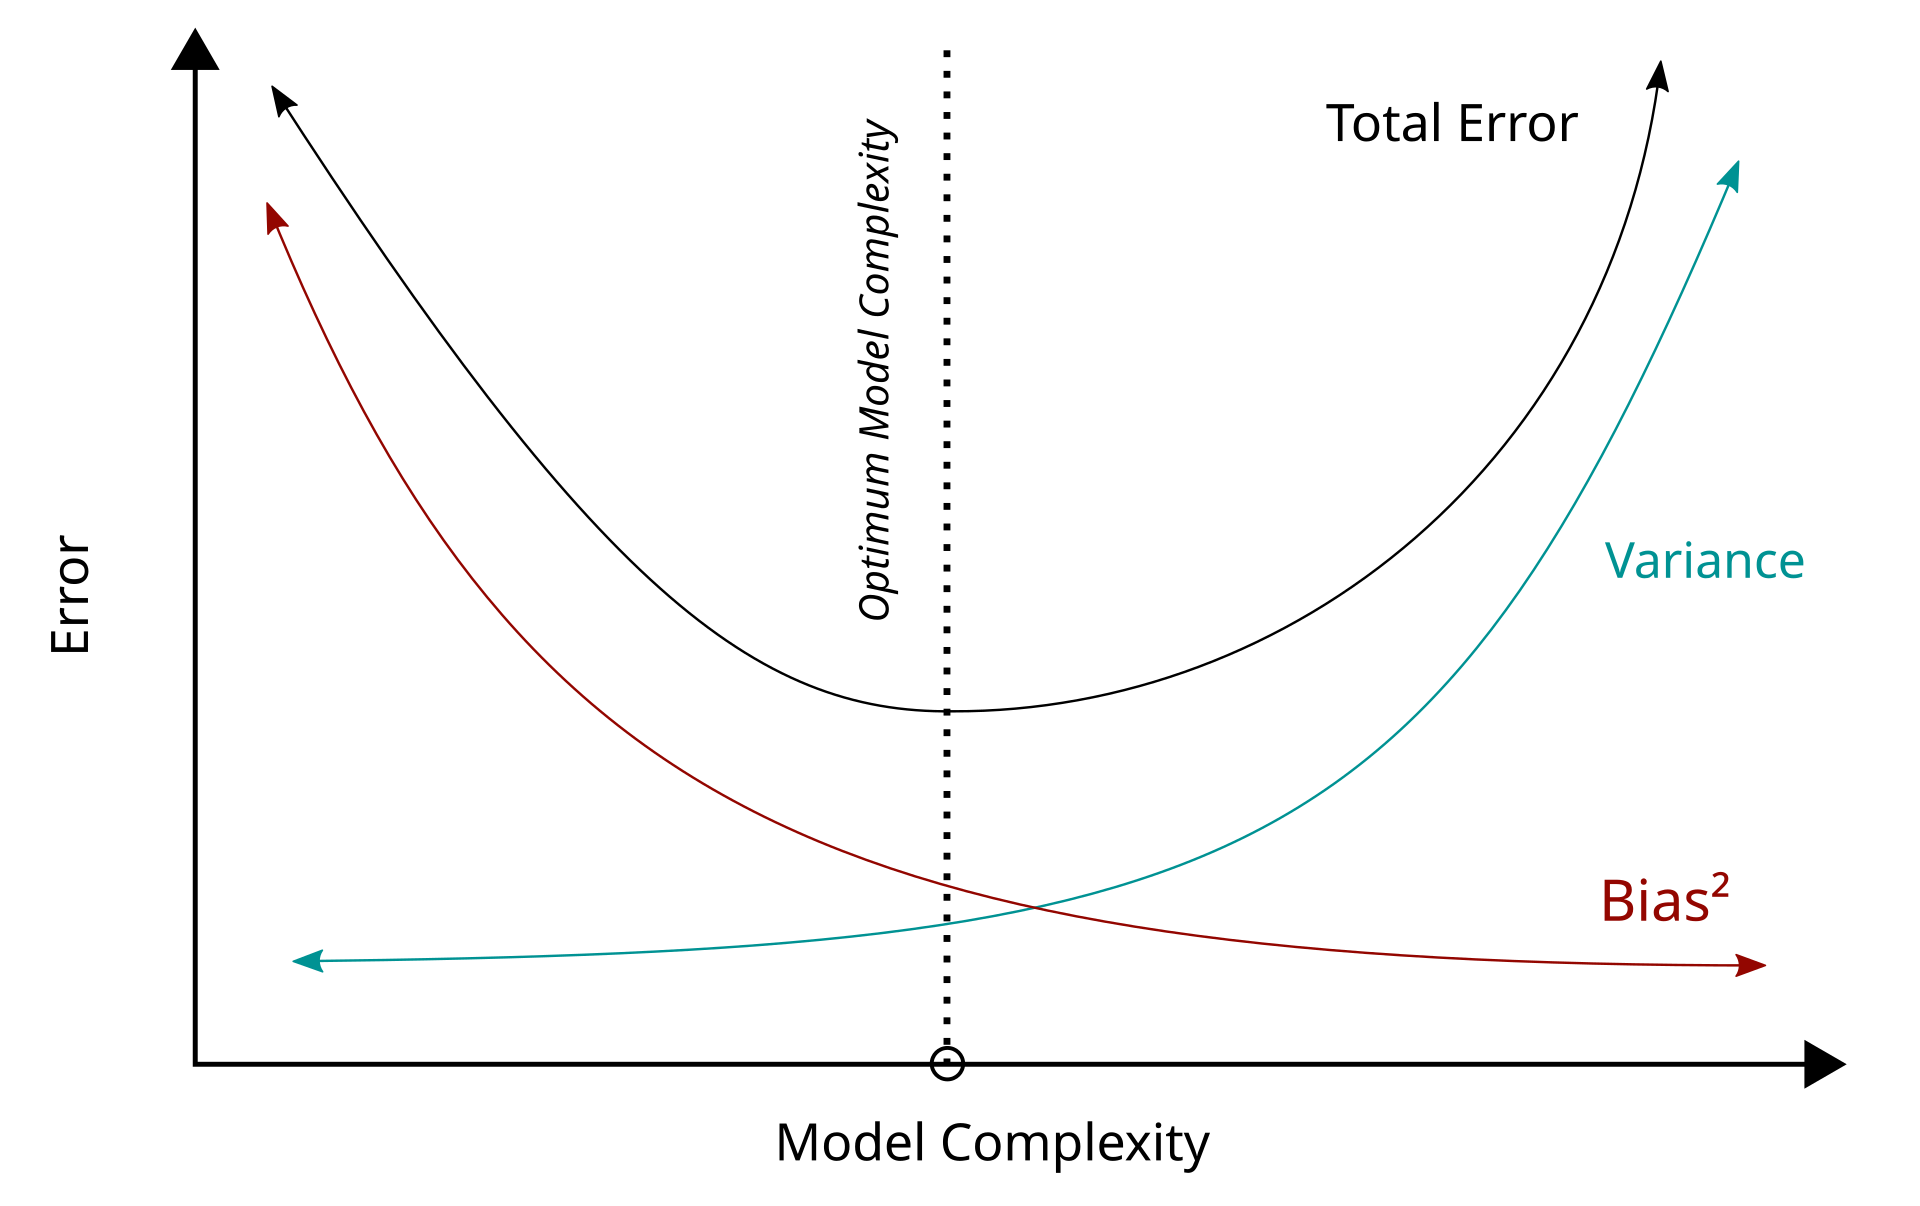
\includegraphics[width=.9\textwidth]{bias-variance-tradeoff.png}
\end{center}

\section{Evaluation / performance metrics for classifiers}
\subsection{ROC AUC}
belongs to the class of ranking metrics or discrimination measures. Why? because it evaluates how well a classifier ranks positive instances above negative ones, rather than directly measuring error rates.

It is a threshold-dependent metric.

\paragraph{True Positive and False Positive Rate} are functions of the threshold $t$.
$$ TPR = \frac{TP}{TP + FN} $$
This is like $P(\hat y = 1 \mid y = 1)$.

The false positive rate meanwhile is $P(\hat y = 1 \mid y = 0)$. I.e., $\frac{FP}{FP + TN}$.

Why are they functions of $t$? $t$ is a decision boundary that determines how a classifier assigns labels based on the predicted scores (e.g., probabilities from a logistic regression model). In other words,
$$ \hat y = \begin{cases}
    1, & \text{if score} > t \\
    0, & \text{otherwise.}
\end{cases} $$

If we lower $t$, then more samples are classified as positive, thus $TPR$ and $FPR$ increase. I.e., $TPR(t)$ and $FPR(t)$ are monotonically decreasing. Furthermore, $TPR(0) = FPR(0) = 1$ and $TPR(1) = FPR(1) = 0$. Due to the monotonicity, $TPR$ and $FPR$ can be considered functions of each other.

\paragraph{The ROC (Receiver Operating Characteristic) curve} is a parametric plot of True Positive Rate ($TPR$) as a function of False Positive Rate ($FPR$).

\begin{center}
    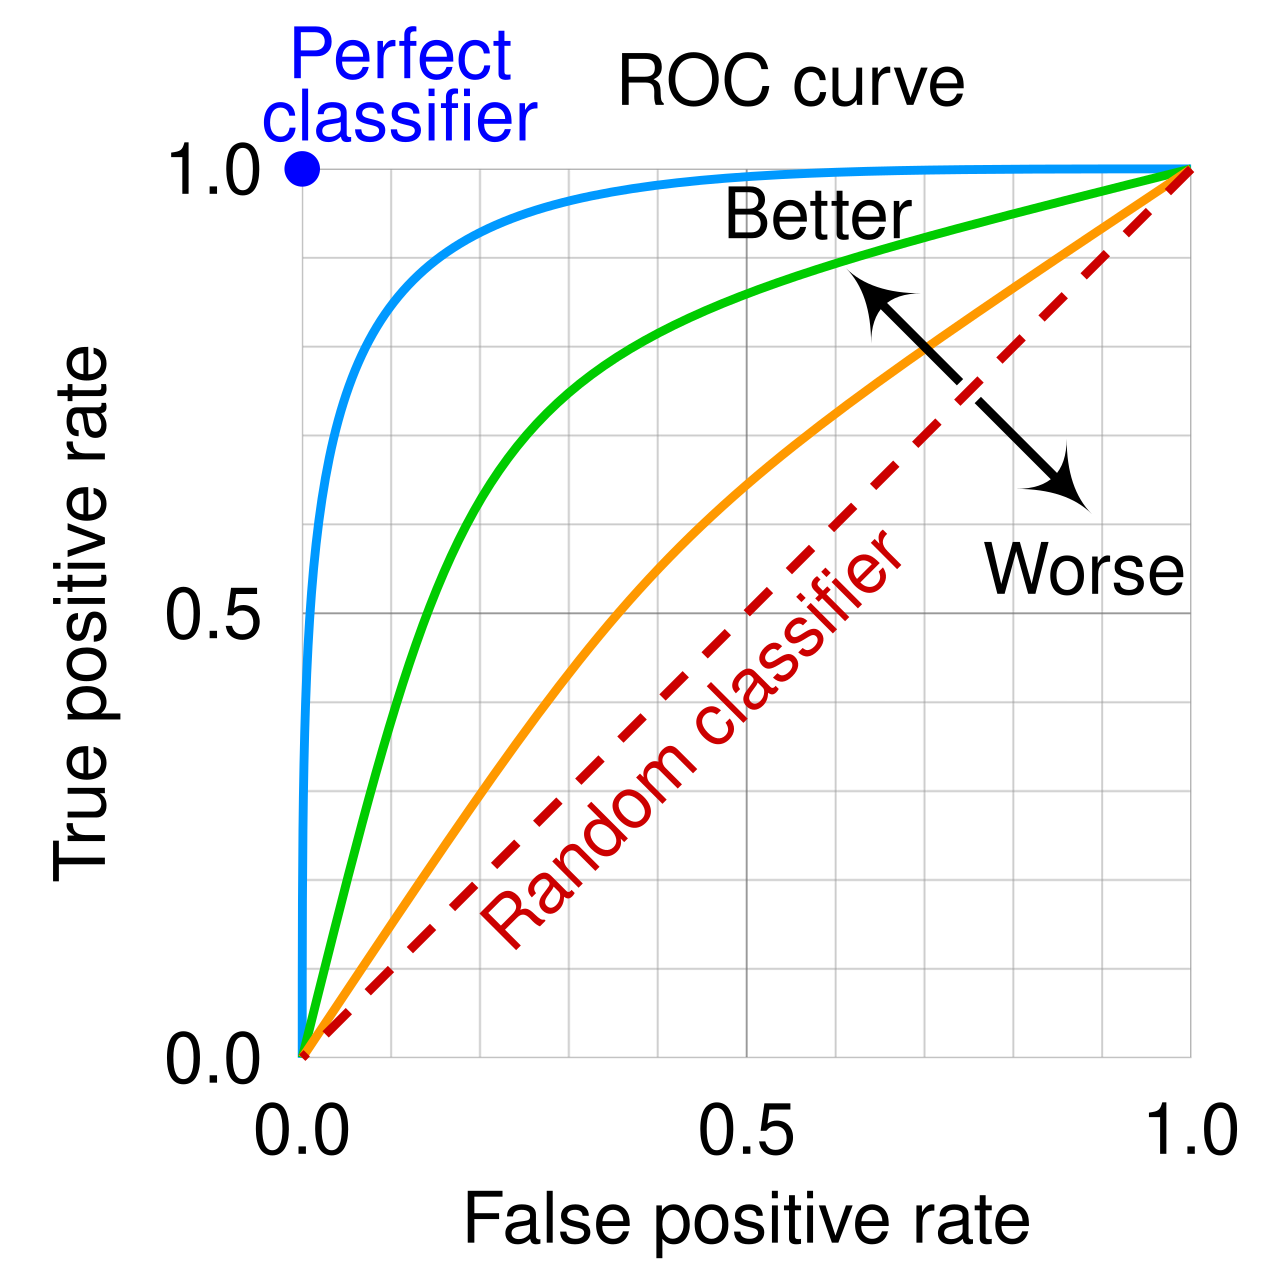
\includegraphics[width=.3\textwidth]{Roc_curve.png}    
\end{center}

\paragraph{$AUC$} stands for area under curve. $ROC$ $AUC$ is obviously
$$ AUC = \int_0^1 TPR \, dFPR $$

\paragraph{How to pick $t$?}
\begin{itemize}
    \item Do you want to maximize TPR (sensitivity) while allowing some false positives?
    \item Do you want to minimize FPR (1-specificity) while keeping TPR high?
    \item Do you want to balance both?
\end{itemize}

\paragraph{$TNR$ (aka specificity) and $FNR$?}
note
\begin{itemize}
    \item $TNR = 1-FPR$
    \item $FNR = 1-TPR$
    \item If true negatives are important (e.g., specificity in medical screening), you might prefer to use the Precision-Recall Curve instead of ROC.
    \item If false negatives are costly (e.g., missing fraud cases), focusing on recall or the F1-score might be better.
\end{itemize}

\subsection{F1 score} is defined as
$$ F1 = \frac{2 \cdot Precision \cdot Recall}{Precision+Recall}, $$
i.e. the harmonic mean of Precision and Recall. It is a function of $t$. Here,
\begin{itemize}
    \item $Precision = Positive\ Predictive\ Value = PPV = \frac{TP}{TP + FP} = P(y = 1 \mid \hat y=1)$
    \item $Recall = TPR = \frac{TP}{TP + FN} = P(\hat y=1 \mid y=1)$
\end{itemize}

\begin{center}
    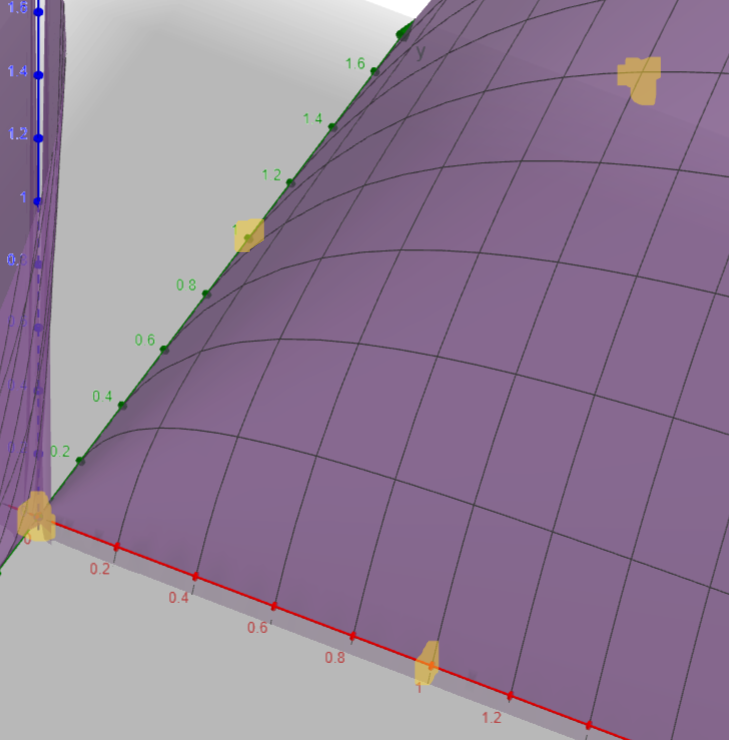
\includegraphics[width=.3\textwidth]{harmonic_mean.png}
\end{center}

Note: the F1-score is generally not monotonous in the threshold $t$.

Choosing $t$ to maximize F1 is a reasonable and common approach, especially in scenarios where you want to find a balance between precision and recall.

\subsection{\texorpdfstring{$R^2$, i.e., coefficient of determination}{R2, i.e., coefficient of determination}}
defn.
$$ R^2 = 1 - \frac{\sum_i (y_i - \hat y_i)^2}{\sum_i (y_i - \bar y)^2} $$
This is the square of the Pearson correlation coefficient
$$ r = \frac{\Cov(y,\hat y)}{\sqrt{\Var(y) \Var(\hat y)}}. $$
Due to the Cauchy--Schwarz inequality, $r$ always lies between $-1$ and $+1$.

\section{Clustering}
\subsection{K-Means Clustering}
\begin{itemize}
    \item Concept: Divides the data into $k$ clusters, where each data point belongs to the cluster with the nearest mean (centroid).
    \item How it works: Randomly initialize $k$ centroids.
    \item Assign each data point to the nearest centroid. Recalculate centroids based on the mean of assigned points. Repeat until convergence (centroids don't change significantly). Advantages: Simple, fast, works well with large datasets.
    \item Disadvantages: Requires the number of clusters $k$ to be specified in advance, sensitive to initial centroid placement, struggles with non-spherical clusters or varying densities.
\end{itemize}


\section{Reinforcement Learning}
\begin{itemize}
    \item MDP: Markov Decision Process
    \item Bellman equation
    \item the multi-armed bandit problem = one-state Markov decision process
\end{itemize}

\section{Other topics in Data Science}
\subsection{Association Rules}
\begin{itemize}
    \item especially popular in market basket analysis -- like finding out which products are often bought together by customers
    \item Key Metrics in Association Rules
    \begin{itemize}
        \item Support
        \item Confidence
        \item Lift
    \end{itemize}
    \item Uses notation from symbolic logic
\end{itemize}

\appendix
\section{Statistics}
\subsection{p-hacking}
The goal of hypothesis testing is to determine whether there is enough evidence in the data to reject the null hypothesis in favor of the alternative hypothesis, based on a p-value. The p-value represents the probability of obtaining the observed data (or more extreme results) if the null hypothesis is true.

For a hypothesis to be rejected in hypothesis testing, the p-value needs to be lower than a predefined significance level, often denoted as $\alpha$. Typically, $\alpha = 0.05$. It represents the maximum probability of committing a Type I error (rejecting the null hypothesis when it is actually true).

p-value: The probability of obtaining results as extreme as (or more extreme than) the results observed in your sample, assuming the null hypothesis is true.
$$ p=P(\text{Data as extreme or more extreme than observed}\mid H_0) $$

\subsection{Wölbung / Kurtosis}
$$ \beta_2 = \E[(\frac{X-\mu}{\sigma^2})^4] = \frac{\E[(X-\mu)^4]}{\E[(X-\mu)^2]^2}$$
Um das Ausmaß der Wölbung besser einschätzen zu können, wird sie mit der Wölbung einer Normalverteilung verglichen, für die $\beta_2 = 3$ gilt. Der Exzess (auch: Überschusswölbung oder Überkurtosis) ist daher definiert als
$$ \gamma = \beta_2 - 3 $$

Arten von Exzess:
\begin{itemize}
    \item $\gamma < 0$: platykurtisch (flach)
    \item $\gamma = 0$: mesokurtisch (wie Normalverteilung)
    \item $\gamma > 0$: leptokurtisch (spitz)
\end{itemize}



%\addcontentsline{toc}{section}{References}
\printbibliography[heading=bibintoc]

\end{document}